% Created 2016-03-17 Thu 11:23
\documentclass[10pt,t,a4paper]{beamer}
\usepackage[utf8]{inputenc}
\usepackage[T1]{fontenc}
\usepackage{fixltx2e}
\usepackage{graphicx}
\usepackage{longtable}
\usepackage{float}
\usepackage{wrapfig}
\usepackage{rotating}
\usepackage[normalem]{ulem}
\usepackage{amsmath}
\usepackage{textcomp}
\usepackage{marvosym}
\usepackage{wasysym}
\usepackage{amssymb}
\usepackage{hyperref}
\tolerance=1000
\usetheme{BTH_msv}
\author{Mikael Svahnberg\thanks{Mikael.Svahnberg@bth.se}}
\date{2016-03-09}
\title{Development Process \\\\ \texttt{PA14[13]5}}
\hypersetup{
  pdfkeywords={},
  pdfsubject={},
  pdfcreator={Emacs 25.1.50.1 (Org mode 8.2.10)}}
\begin{document}

\maketitle

\section{Classroom}
\label{sec-1}
\begin{frame}[label=sec-1-1]{Software Engineering}
\begin{itemize}
\item IEEE std 610.12:1990 ``IEEE Standard Glossary of Software Engineering Terminology'':
\end{itemize}

\begin{block}{Software Engineering}
The application of a systematic, disciplined, quantifiable approach to the development, operation, and maintenance of software; that is, the application of engineering to software.
\end{block}
\end{frame}

\begin{frame}[fragile,label=sec-1-2]{Software Engineering Process}
 \begin{itemize}
\item \alert{Systematic}
\begin{itemize}
\item Pre-planned, not ad-hoc
\item Thorough
\item Repeatable
\end{itemize}
\item \alert{Disciplined}
\begin{itemize}
\item Following the plan
\item Eyes on target
\end{itemize}
\item \alert{Quantifiable}
\begin{itemize}
\item Measurable
\end{itemize}
\end{itemize}


\begin{itemize}
\item \alert{Development}
\begin{itemize}
\item \texttt{*this}
\end{itemize}
\item \alert{Operation}
\begin{itemize}
\item Deployment is an important part of SE, and must be planned accordingly.
\end{itemize}
\item \alert{Maintenance}
\begin{itemize}
\item 80\% -- 90\% of a system's life span is spent in maintenance.
\end{itemize}
\end{itemize}
\end{frame}
\begin{frame}[label=sec-1-3]{Process vs Project vs Product}
T. Gorschek, A.M. Davis, \emph{Requirements Engineering; In Search of the Dependent Variables}, Information and Software Tecnology 50(2008):67--75.

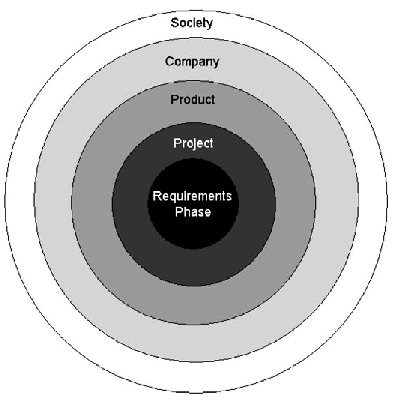
\includegraphics[height=5cm]{./FGorschek_Onion.pdf}

(+ Process, which is not visible in this figure but neatly bisects it.)
\end{frame}
\begin{frame}[shrink=15,label=sec-1-4]{Example of UML Process:}

\begin{block}{Dice Game Machine}
\begin{itemize}
\item On the Machine a player may login, logout or play the game.
\item When playing the game a player rolls two die. If the total number of points is greater than seven the player wins, otherwise the player loses.
\end{itemize}
\end{block}

\begin{block}{Construct}
\begin{itemize}
\item Use Case Diagrams
\item Use Cases
\item Conceptual Model
\item Class Diagram
\item Collaboration Diagram
\item Interaction Diagram
\item Flowcharts?
\item ?? What happened to testing ??
\end{itemize}
\end{block}
\end{frame}
\begin{frame}[label=sec-1-5]{Discussion}
\begin{itemize}
\item What is good with waterfall?
\item Where/How would you do design in Scrum?
\item Where would you do design in Kanban?
\item When should you use which process model?
\item What are their limitations?
\item Does it work to incrementally test a product like this?
\end{itemize}
\end{frame}
% Emacs 25.1.50.1 (Org mode 8.2.10)
\end{document}